%%%%%%%%%%%%%%%%%%%%%%%%%%%%%%%%%%%%%%%%%%%%%%%%%%%%%%%%%%%%%%%%%%%%%%%%%%%%%%%
%                       CARGA DE LA CLASE DE DOCUMENTO                        %
%                                                                             %
% Las opciones admisibles son:                                                %
%      12pt / 11pt            (tamaño del cuerpo de letra; no usar 10pt)      %
%                                                                             %
% catalan/spanish/english     (idioma principal del trabajo)                  %
%                                                                             % 
% french/italian/german...    (si necesitáis usar otro idioma adicional)      %
%                                                                             %
% listoffigures               (El documento incluye un Índice de figuras)     %
% listoftables                (El documento incluye un Índice de tablas)      %
% listofquadres               (El documento incluye un Índice de cuadros)     %
% listofalgorithms            (El documento incluye un Índice de algoritmos)  %
%                                                                             %
%%%%%%%%%%%%%%%%%%%%%%%%%%%%%%%%%%%%%%%%%%%%%%%%%%%%%%%%%%%%%%%%%%%%%%%%%%%%%%%

\documentclass[11pt,spanish,listoffigures,listoftables]{tfgetsinf}

%%%%%%%%%%%%%%%%%%%%%%%%%%%%%%%%%%%%%%%%%%%%%%%%%%%%%%%%%%%%%%%%%%%%%%%%%%%%%%%
%                     CODIFICACIÓN DEL ARCHIVO FUENTE                         %
%                                                                             %
%    Windows suele usar 'ansinew'                                             %
%    en Linux es posible que sea 'latin1' o 'latin9'                          %
%    Pero lo más recomendable es usar utf8 (unicode 8)                        %
%                                          (si vuestro editor lo permite)     % 
%%%%%%%%%%%%%%%%%%%%%%%%%%%%%%%%%%%%%%%%%%%%%%%%%%%%%%%%%%%%%%%%%%%%%%%%%%%%%%%

\usepackage[utf8]{inputenc} 


%%%%%%%%%%%%%%%%%%%%%%%%%%%%%%%%%%%%%%%%%%%%%%%%%%%%%%%%%%%%%%%%%%%%%%%%%%%%%%%
%                       OTROS PAQUETES Y DEFINICIONES                         %
%                                                                             %
%%%%%%%%%%%%%%%%%%%%%%%%%%%%%%%%%%%%%%%%%%%%%%%%%%%%%%%%%%%%%%%%%%%%%%%%%%%%%%%

\usepackage{glossaries}
\usepackage{textcomp}
\usepackage{booktabs}
\usepackage{float}
\usepackage{enumitem}
\usepackage{graphicx}
\usepackage{subcaption}
\usepackage{tabularx}
\usepackage{pgfplots}
\pgfplotsset{compat=1.18}

% Listings para código
\usepackage{listings}
\lstset{
  basicstyle=\ttfamily\small,
  frame=single,
  breaklines=true,
  postbreak=\mbox{\textcolor{gray}{$\hookrightarrow$}\space},
  columns=fullflexible,
  keepspaces=true,
  numbers=none
}

% Bibliografía
\usepackage[backend=biber,style=numeric,sorting=none]{biblatex}
\addbibresource{bibliografia.bib}

% Hyperref siempre al final
\usepackage{hyperref}
\hypersetup{
  colorlinks=true,
  linkcolor=black,
  urlcolor=cyan,
  citecolor=black
}
%%%%%%%%%%%%%%%%%%%%%%%%%%%%%%%%%%%%%%%%%%%%%%%%%%%%%%%%%%%%%%%%%%%%%%%%%%%%%%%
%                          DATOS DEL TRABAJO                                  %
%                                                                             %
% título alumno, titor y curso académico                                      %
%%%%%%%%%%%%%%%%%%%%%%%%%%%%%%%%%%%%%%%%%%%%%%%%%%%%%%%%%%%%%%%%%%%%%%%%%%%%%%%

\title{Traducción Automática de Español a Esperanto}
\author{Gómez Corral, Miquel}
% \tutor{No}
% \curs{MUIARFID}

%%%%%%%%%%%%%%%%%%%%%%%%%%%%%%%%%%%%%%%%%%%%%%%%%%%%%%%%%%%%%%%%%%%%%%%%%%%%%%%
%                     PARAULES CLAU/PALABRAS CLAVE/KEY WORDS                  %
%                                                                             %
% Independentment de la llengua del treball, s'hi han d'incloure              %
% les paraules clau i el resum en els tres idiomes                            %
%%%%%%%%%%%%%%%%%%%%%%%%%%%%%%%%%%%%%%%%%%%%%%%%%%%%%%%%%%%%%%%%%%%%%%%%%%%%%%%

\keywords{
    Traducción de textos; español; esperanto; Transformers; LLMs
} % Paraules clau 
{
   Traducción de textos; 
} % Palabras clave
{
    Text clasification.
} % Key words


%%%%%%%%%%%%%%%%%%%%%%%%%%%%%%%%%%%%%%%%%%%%%%%%%%%%%%%%%%%%%%%%%%%%%%%%%%%%%%%
%                                                                             %
%                              INICI DEL DOCUMENT                             %
%                                                                             %
%%%%%%%%%%%%%%%%%%%%%%%%%%%%%%%%%%%%%%%%%%%%%%%%%%%%%%%%%%%%%%%%%%%%%%%%%%%%%%%

\begin{document} 


%%%%%%%%%%%%%%%%%%%%%%%%%%%%%%%%%%%%%%%%%%%%%%%%%%%%%%%%%%%%%%%%%%%%%%%%%%%%%%%
%              RESUMENES DEL TFG EN VALENCIA, CASTELLA I ANGLES               %
%%%%%%%%%%%%%%%%%%%%%%%%%%%%%%%%%%%%%%%%%%%%%%%%%%%%%%%%%%%%%%%%%%%%%%%%%%%%%%%


% \begin{abstract}[spanish]

% \end{abstract}

%%%%%%%%%%%%%%%%%%%%%%%%%%%%%%%%%%%%%%%%%%%%%%%%%%%%%%%%%%%%%%%%%%%%%%%%%%%%%%%
%                                                                             %
%                              CONTENIDO DEL TREBAJO                          %
%                                                                             %
%%%%%%%%%%%%%%%%%%%%%%%%%%%%%%%%%%%%%%%%%%%%%%%%%%%%%%%%%%%%%%%%%%%%%%%%%%%%%%%

%%%%%%%%%%%%%%%%%%%%%%%%%%%%%%%%%%%%%%%%%%%%%%%%%%%%%%%%%%%%%%%%%%%%%%%%%%%%%%%
%                                  ÍDNICE                                     %
%%%%%%%%%%%%%%%%%%%%%%%%%%%%%%%%%%%%%%%%%%%%%%%%%%%%%%%%%%%%%%%%%%%%%%%%%%%%%%%
% \clearpage
% \tableofcontents
% \listoffigures
% \listoftables


\mainmatter

\chapter{Introducción y Dataset}
Este trabajo aborda la traducción automática de textos del español al esperanto. Se utilizarán modelos basados en la arquitectura Transformer y LLMs preentrenados, adaptados mediante técnicas de fine-tuning y transfer learning.

\section{Dataset}
El dataset elegido ha sido CCMatrix \cite{schwenk-2019}, un corpus de pares de oraciones alineadas en múltiples idiomas extraídas mediante crawling web. Contiene más de 10 millones de pares en más de 100 idiomas, incluyendo lenguas mayoritarias y minoritarias.

Para este trabajo nos interesan los pares español-esperanto: más de 5.7 millones de frases, con aproximadamente 80 millones de tokens en español y 73.3 millones en esperanto.

\subsection{Limitaciones y tratamiento del dataset}
El dataset original es demasiado grande para el alcance de este trabajo. Para usarlo de manera efectiva, primero se han filtrado los pares con artefactos de HTML y otros efectos del crawling. Después, se ha reducido al 5\% del total, seleccionando aleatoriamente los pares. Finalmente, se ha dividido en entrenamiento (70\%), validación (15\%) y test (15\%):
\begin{itemize}
    \item Entrenamiento: $201\;000$ pares de oraciones.
    \item Validación: $43\;000$ pares de oraciones.
    \item Test: $43\;000$ pares de oraciones.
\end{itemize}

Además, en cada experimento se han eliminado pares demasiado largos según cada tokenizador, quedando reportado en el código.

\section{Hardware utilizado}
Los experimentos se han realizado en mi máquina personal: GPU NVIDIA RTX 5070 (12 GB VRAM), procesador AMD Ryzen 9 9000X, 64 GB de RAM y Ubuntu 24.04 LTS.

Todos los modelos han podido ser entrenados y evaluados sin problemas. La única limitación ha sido el tiempo de entrenamiento, que en algunos casos ha sido elevado (+24 ctrl alt texhoras).

%%%%%%%%%%%%%%%%%%%%%%%%%%%%%%%%%%%%%%%%%%%%%%%%%%%%%%%%%%%%%%%%%%%%%%%%%%%%%
%                        Notebooks base                                     %
%%%%%%%%%%%%%%%%%%%%%%%%%%%%%%%%%%%%%%%%%%%%%%%%%%%%%%%%%%%%%%%%%%%%%%%%%%%%%
\chapter{Notebooks base}
\section{Modificaciones realizadas}
Comentamos brevemente los cambios realizados en los notebooks base proporcionados para conseguir usar nuestro dataset e incluir la métrica COMET \cite{rei-etal-2020-comet-hf}.

\subsection{Dataset}
El dataset se ha descargado en formato CSV y se ha creado una clase envoltorio para adaptarlo al formato HuggingFace \cite{huggingface-2025-trl-docs}. Con Pandas \cite{pandas-2025}, se ha cargado el CSV, se ha separado en conjuntos de entrenamiento, validación y test, y se ha instanciado la clase.

\subsection{Métrica COMET}
La métrica COMET requiere la oración fuente, objetivo y predicha. Se ha modificado el código de evaluación para guardar también la oración fuente (las otras ya estaban). \noindent  Las métricas COMET se reportan multiplicadas por 99 para facilitar las comparaciones (su rango habitual es $[0, 1]$).

\section{Resultados base}

Los resultados de los modelos base se muestran en la Tabla~\ref{tab:resultados_base} con sus métricas BLEU y COMET: NLLB Baseline (\texttt{ES-EO-LL3.4\_NMT\_NLLB\_Baseline.ipynb}), NLLB Fine-Tuned (\texttt{ES-EO-L3.4\_NMT\_NLLB\_Finetuning.ipynb}), LLAMA Prompting (\texttt{ES-EO-L3.5\_NMT\_LLAMA\\\_Prompting.ipynb}) y LLAMA Fine-Tuned (\texttt{ES-EO-L3.5\_NMT\_LLAMA\_Finetuning.ipynb}).

\begin{table}[H]
\footnotesize
\centering
\begin{tabular}{lrr}
	\toprule
	\textbf{Modelo} & \textbf{BLEU} & \textbf{COMET} \\
	\midrule
	NLLB Baseline & 19.10 & 80.06 \\
	NLLB Fine-Tuned & 25.37 & 81.76 \\
	LLAMA Prompting & 4.64 & 60.62 \\
	LLAMA Fine-Tuned & 22.76 & 79.10 \\
	\bottomrule
\end{tabular}
\caption{Comparación de resultados para los modelos base usando las métricas BLEU y COMET.}
\label{tab:resultados_base}
\end{table}

\noindent El modelo NLLB Fine-Tuned ha obtenido los mejores resultados en ambas métricas, seguido por LLAMA Fine-Tuned. El modelo NLLB Baseline también ha mostrado un rendimiento aceptable, mientras que LLAMA Prompting ha obtenido los peores resultados.

%%%%%%%%%%%%%%%%%%%%%%%%%%%%%%%%%%%%%%%%%%%%%%%%%%%%%%%%%%%%%%%%%%%%%%%%%%%%%%%
%                           TÉCNOLOGÍAS PLANTEADAS                            %
%%%%%%%%%%%%%%%%%%%%%%%%%%%%%%%%%%%%%%%%%%%%%%%%%%%%%%%%%%%%%%%%%%%%%%%%%%%%%%%
\chapter{Ampliación de modelos}

%%%%%%%%%%%%%%%%%%%%%%%%%%%%%%%%%%%%%%%%%%%%%%%%%%%%%%%%%%%%%%%%%%%%%%%%
\section{Modelo extra 1: \textit{mt5-large}}
El modelo \texttt{mt5-large} \cite{google-2024-mt5} es un transformer preentrenado por Google con el dataset mC4 \cite{raffel-etal-2019-c4} (versión multilingüe de C4). Es multilingüe pero no especializado en traducción, por lo que requiere de fine-tuning.

Las modificaciones técnicas realizadas en los notebooks para adaptar este modelo, se pueden ver en el Apéndice~\ref{appendix:ajustes_notebooks}, Sección~\ref{sec:ajustes_mt5}.

Resultados iniciales con fine-tuning usando BLEU como objetivo de entrenamiento (\texttt{ES-EO-L3.4\_NMT\_mt5-large\_Finetuning-bleu-base.ipynb}): 

\begin{table}[H]
\centering
\begin{tabular}{lr}
	\toprule
	\textbf{Métrica} & \textbf{Valor} \\
	\midrule
	BLEU & 8.88 \\
	COMET & 66.95 \\
	\bottomrule
\end{tabular}
\caption{Resultados del modelo mt5-large con fine-tuning inicial.}
\label{tab:mt5_baseline}
\end{table}

\section{Modelo extra 2: \textit{LLAMA-3-8B}}
Se ha probado LLAMA 3 (8B parámetros) como alternativa más reciente al LLAMA 2 usado en los notebooks base. Se ha usado por ser un modelo más moderno pero que mantiene un buen tamaño en comparación con LLAMA 2 (7B parámetros).

Para las modificaciones técnicas realizadas en los notebooks para adaptar este modelo, ver Apéndice~\ref{appendix:ajustes_notebooks}, Sección~\ref{sec:ajustes_llama3}.

Resultados sin fine-tuning (\texttt{ES-EO-L3.5\_NMT\_LLAMA-3\_Prompting.ipynb}):

\begin{table}[H]
\centering
\begin{tabular}{lr}
	\toprule
	\textbf{Métrica} & \textbf{Valor} \\
	\midrule
	BLEU & 7.98 \\
	COMET & 66.24 \\
	\bottomrule
\end{tabular}
\caption{Resultados del modelo LLAMA-3-8B sin fine-tuning.}
\label{tab:llama3_prompting}
\end{table}

\section{Exploración de parámetros}
Para todos los puntos de esta sección, se ha utilizado el modelo \textit{mt5-large}. Tanto para la exploración de hiperparámetros, como para las inferencias. Se ha seleccionado este modelo por ser algo más pequeño que LLAMA-3, y porque los transformers base fine-tuneados, han conseguido mejor puntuación en la tarea.

\subsection{Métricas adicionales}
Se ha decidido experimentar con la métrica \textbf{CHRF} \cite{evaluate-metric-2025-chrf}, por ser diferente a las otras dos. CHRF está basada en n-gramas de caracteres, y su rango de valores se encuentra en $[0, 100]$, con valores $>60$ indicando muy buen rendimiento. Se ha usado como métrica de evaluación durante el fine-tuning. 
\subsection{Entrenamiento}
Para mejorar el entrenamiento base de NLLB, se han modificado los siguientes hiperparámetros (\texttt{ES-EO-L3.4\_NMT\_mt5-large\_Finetuning-chrf-base.ipynb} y \texttt{ES-EO-L3.4\_NMT\\\_mt5-large\_Finetuning-chrf-less\_data.ipynb}):

\begin{table}[H]
\centering
\begin{tabular}{lrr}
	\toprule
	\textbf{Hiperparámetro} & \textbf{Base} & \textbf{Mejorado} \\
	\midrule
	Batch size & 4 & 8 \\
	max\_tok\_length & 16 & 64 \\
	max\_epoch & 5 & 10 \\
	Lora: r & 16 & 32 \\
	Lora: alpha & 32 & 64 \\
	Lora: dropout & 0.05 & 0.1 \\
	Generation beams & 1 & 5 \\
	\bottomrule
\end{tabular}
\caption{Hiperparámetros explorados para el entrenamiento.}
\label{tab:hyperparams}
\end{table}

Por las limitaciones que nos da haber usado tantos datos, solo se ha realizado este gran experimento (se da por entendido el cómo ajustar hiperparámetros). Ahora, se ha decidido hacer un experimento reduciendo el dataset de entrenamiento al 0.5\% (28 709 pares), para ver si se podía mejorar el rendimiento. Con esta configuración y usando la métrica CHRF, se han conseguido las métricas:
\begin{table}[H]
\centering
\begin{tabular}{lrr}
	\toprule
	\textbf{Métrica} & \textbf{5\% datos} & \textbf{0.5\% datos}\\
	\midrule
	BLEU & 23.26 & 20.72\\
	COMET & 74.61 & 72.21  \\
	CHRF & 50.25 & 47.12 \\
	\bottomrule
\end{tabular}
\caption{Resultados modelo mt5-large f.t. usando la métrica CHRF y mejores hiperparámetros con 5\% datos y 0.5\% datos.}
\label{tab:mt5_large_chrf}
\end{table}

Como vemos, el rendimiento ha mejorado notoraiablemente respecto al entrenamiento base, pero se ha perdido algo de calidad al reducir los datos. Aun así, el modelo con menos datos sigue superando al modelo base.

\subsection{Inferencia}
Para la inferencia, se ha usado como base el modelo resultante del entrenamiento anterior (5\% datos). Se han comparado estrategias deterministas y estocásticas (\texttt{ES-EO-L3.4\\\_NMT\_mt5-large\_Finetuning-chrf-inference.ipynb}). Las deterministas (greedy y beam search) generan siempre la misma salida, mientras que las estocásticas (sampling) introducen aleatoriedad mediante temperatura, top-k y top-p.

Se han probado cuatro configuraciones: \textbf{greedy} (sin beams, determinista), \textbf{beam} (5 beams, determinista), \textbf{sampling} (3 beams, temperatura 0.2, top-k 30, top-p 0.9) y \textbf{random} (3 beams, temperatura 0.6, top-k 30, top-p 0.9).

\begin{table}[H]
\footnotesize
\centering
\begin{tabular}{lrrr}
	\toprule
	\textbf{Estrategia} & \textbf{BLEU} & \textbf{COMET} & \textbf{CHRF} \\
	\midrule
	Greedy & 23.25 & 74.59 & 50.23 \\
	Beam & 23.51 & 76.04 & 52.26 \\
	Sampling & 23.87 & 75.99 & 52.01 \\
	Random & 23.78 & 75.94 & 52.08 \\
	\bottomrule
\end{tabular}
\caption{Comparación de estrategias de inferencia para mt5-large.}
\label{tab:inference_strategies}
\end{table}

Los resultados son muy similares entre todas las estrategias, sin diferencia estadística significativa entre los experimentos que usan \texttt{beams > 1}. La única diferencia notable es que estas tienden a obtener mejores puntuaciones que usar un solo beam (\texttt{beam = 1}).

Por reproducibilidad, se selecciona \textbf{beam search} como estrategia final al ser determinista y obtener el mejor COMET.

\section{Resultados obtenidos y conclusiones}
La Figura~\ref{fig:resultados_finales} muestra la comparación de todos los modelos evaluados en este trabajo.

\begin{figure}[H]
\centering
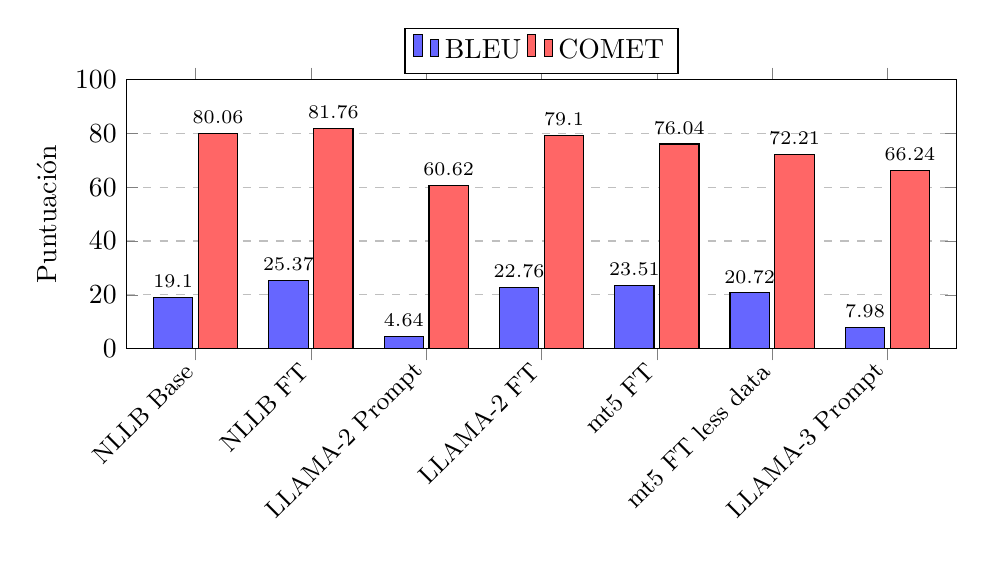
\begin{tikzpicture}
\begin{axis}[
    ybar,
    bar width=0.5cm,
    width=\textwidth,
    height=5cm,
    ylabel={Puntuación},
    symbolic x coords={NLLB Base, NLLB FT, LLAMA-2 Prompt, LLAMA-2 FT, mt5 FT, mt5 FT less data, LLAMA-3 Prompt},
    xtick=data,
    x tick label style={rotate=45, anchor=east, font=\small},
    legend style={at={(0.5,1.02)}, anchor=south, legend columns=2},
    ymin=0,
    ymax=100,
    ymajorgrids=true,
    grid style=dashed,
    enlarge x limits=0.1,
    nodes near coords,
    nodes near coords align={vertical},
    every node near coord/.append style={font=\scriptsize},
]

% BLEU scores
\addplot[fill=blue!60] coordinates {
    (NLLB Base, 19.10)
    (NLLB FT, 25.37)
    (LLAMA-2 Prompt, 4.64)
    (LLAMA-2 FT, 22.76)
    (mt5 FT, 23.51)
    (mt5 FT less data, 20.72)
    (LLAMA-3 Prompt, 7.98)
};

% COMET scores
\addplot[fill=red!60] coordinates {
    (NLLB Base, 80.06)
    (NLLB FT, 81.76)
    (LLAMA-2 Prompt, 60.62)
    (LLAMA-2 FT, 79.10)
    (mt5 FT, 76.04)
    (mt5 FT less data, 72.21)
    (LLAMA-3 Prompt, 66.24)
};

\legend{BLEU, COMET}

\end{axis}
\end{tikzpicture}
\caption{Comparación de resultados finales de todos los modelos usando BLEU y COMET. FT = Fine-Tuned, Prompt = Prompting.}
\label{fig:resultados_finales}
\end{figure}


\noindent El mejor modelo es \textbf{NLLB Fine-Tuned} con BLEU 25.37 y COMET 81.76. El modelo \textbf{mt5-large} con los hiperparámetros optimizados alcanza un rendimiento competitivo (BLEU 23.51, COMET 76.04), superando a LLAMA-2 Fine-Tuned en BLEU. Los modelos sin fine-tuning (prompting) obtienen resultados significativamente peores.

%%%%%%%%%%%%%%%%%%%%%%%%%%%%%%%%%%%%%%%%%%%%%%%%%%%%%%%%%%%%%%%%%%%%%%%%%%%%%%%
%                                                                             %
%                                BIBLIOGRAFIA                                 %
%                                                                             %
%%%%%%%%%%%%%%%%%%%%%%%%%%%%%%%%%%%%%%%%%%%%%%%%%%%%%%%%%%%%%%%%%%%%%%%%%%%%%%%
\cleardoublepage
\printbibliography

%%%%%%%%%%%%%%%%%%%%%%%%%%%%%%%%%%%%%%%%%%%%%%%%%%%%%%%%%%%%%%%%%%%%%%%%%%%%%%%
%                                                                             %
%                                 APÉNDICESS                                  %
%                                                                             %
%%%%%%%%%%%%%%%%%%%%%%%%%%%%%%%%%%%%%%%%%%%%%%%%%%%%%%%%%%%%%%%%%%%%%%%%%%%%%%%

\APPENDIX
%%%%%%%%%%%%%%%%%%%%%%%%%%%%%%%%%%%%%%%%%%%%%%%%%%%%%%%%%%%%%%%%%%%%%%%%%%%%%%
%                       AJUSTES DE LOS NOTEBOOKS                             %
%%%%%%%%%%%%%%%%%%%%%%%%%%%%%%%%%%%%%%%%%%%%%%%%%%%%%%%%%%%%%%%%%%%%%%%%%%%%%%

\chapter{Ajustes de los notebooks}
\label{appendix:ajustes_notebooks}

Este apéndice detalla las modificaciones técnicas realizadas en los notebooks para adaptar los modelos adicionales (mt5-large y LLAMA-3-8B) a la tarea de traducción español-esperanto.

\section{Ajustes del modelo mt5-large}
\label{sec:ajustes_mt5}

\begin{itemize}
  \item \textbf{Target modules de LoRA}: \texttt{['q', 'k', 'v', 'o']} para las capas de atención.
  \item \textbf{Instrucciones textuales}: Formato \texttt{"Translate Spanish to Esperanto: [texto]"} en lugar de tokens especiales de idioma.
  \item \textbf{Filtro de tokens}: Clipping de los IDs al rango \texttt{[0, vocab\_size-1]} para evitar errores con tokens inválidos. Por alguna razón el modelo genera IDs fuera de rango por errores durante el entrenamiento.
\end{itemize}

\section{Ajustes del modelo LLAMA-3-8B}
\label{sec:ajustes_llama3}

\begin{itemize}
  \item \textbf{Padding manual}: Implementación de padding por batch con máscaras de atención explícitas.
  \item \textbf{Parámetros de generación}: Uso de \texttt{max\_new\_tokens=128} y \texttt{min\_new\_tokens=10} en lugar de \texttt{max\_length}.
  \item \textbf{Formato del prompt}: Estructura \texttt{"Translate the following Spanish text to \\Esperanto:\textbackslash n\textbackslash nSpanish: [texto]\textbackslash nEsperanto:"} para zero-shot prompting.
\end{itemize}

%%%%%%%%%%%%%%%%%%%%%%%%%%%%%%%%%%%%%%%%%%%%%%%%%%%%%%%%%%%%%%%%%%%%%%%%%%%%%%
%                       EJEMPLOS DE CADA TIPO DE FACTURA                     %
%%%%%%%%%%%%%%%%%%%%%%%%%%%%%%%%%%%%%%%%%%%%%%%%%%%%%%%%%%%%%%%%%%%%%%%%%%%%%%


\chapter{Apéndice correspondencia notebooks}
\label{appendix:notebooks}
Aquí se incluye la descripción de cada notebook y qué contenidos tiene. Todos parten de los notebooks base proporcionados, con las modificaciones necesarias para usar nuestro dataset y la métrica COMET. Se incluye en el repositorio una carpeta \texttt{app} con la clase Dataset personalizada y la configuración.
\begin{enumerate}
	\item Process-dataset: Primer pre-procesado, filtrado y división del dataset.
	\item ES-EO-LL3.4\_NMT\_NLLB\_Baseline: NLLB Baseline con nuestro dataset.
	\item ES-EO-L3.4\_NMT\_NLLB\_Finetuning: NLLB Fine-Tuned con nuestro dataset.
	\item ES-EO-L3.5\_NMT\_LLAMA\_Prompting: LLAMA Prompting con nuestro dataset.
	\item ES-EO-L3.5\_NMT\_LLAMA\_Finetuning: LLAMA Fine-Tuned con nuestro dataset.
	\item ES-EO-L3.5\_NMT\_LLAMA-3\_Prompting: LLAMA-3-8B Prompting con nuestro dataset.
	\item ES-EO-L3.4\_NMT\_mt5-large\_Baseline: mt5-large SIN finetunear, con nuestro dataset.
	\item ES-EO-L3.4\_NMT\_mt5-large\_Finetuning-bleu-base: mt5-large Fine-Tuned \textit{básico} usando BLEU con nuestro dataset.
	\item ES-EO-L3.4\_NMT\_mt5-large\_Finetuning-chrf-base: mt5-large Fine-Tuned \textit{mejorado} usando CHRF con nuestro dataset.
	\item ES-EO-L3.4\_NMT\_mt5-large\_Finetuning-chrf-less\_data: mt5-large Fine-Tuned \textit{mejorado} usando CHRF con nuestro dataset pero usando una versión aún más reducida de los datos (0.5\% en vez de 5\%).
	\item ES-EO-L3.4\_NMT\_mt5-large\_Finetuning-chrf-inference: mt5-large Fine-Tuned \textit{mejorado} (en verdad es el modelo resultante del caso anterior) probando hiperparámetros para validación, con nuestro dataset.
\end{enumerate}


%%%%%%%%%%%%%%%%%%%%%%%%%%%%%%%%%%%%%%%%%%%%%%%%%%%%%%%%%%%%%%%%%%%%%%%%%%%%%%%
%                              FIN DEL DOCUMENTO                              %
%%%%%%%%%%%%%%%%%%%%%%%%%%%%%%%%%%%%%%%%%%%%%%%%%%%%%%%%%%%%%%%%%%%%%%%%%%%%%%%
\end{document}

